\lecture{16}{27 Nov.}{}

Last time we built the Doob martingale of a graph parameter and stated Azuma's inequality (\thmref{thm:azuma}). This lecture proves it, isolates the property of \(f\) that makes the increments of the Doob martingale bounded (being \emph{Lipschitz}), and applies the result to the chromatic number of \(G(n,p)\). The outcome is the Shamir--Spencer theorem: \(\chi(G(n,p))\) lies in an interval of length \(O(\sqrt{n})\) with high probability, although the proof does not say where that interval is. We then start locating it for \(p = \frac{1}{2}\).

\begin{moral}
    Azuma's inequality is Chernoff's bound with independence replaced by the martingale condition. To apply it to \(f(G)\), we only need to check that changing one piece of \(G\) (an edge, or the edges at one vertex) changes \(f\) by at most a constant.
\end{moral}

\subsection{Proof of Azuma's Inequality}\label{sec:azuma-proof}

The proof follows that of \autoref{thm:chernoff-general}: apply Markov's inequality to \(e^{\alpha X_{m}}\) and bound \(\mathbb{E}[e^{\alpha X_{m}}]\). There, \(\mathbb{E}[e^{\lambda S}]\) split into a product by independence. Here the increments need not be independent, so we peel them off one at a time, conditioning on the past. Besides \autoref{fact:tower}, we need one more property of conditional expectation.

\begin{fact}[Taking out what is known]\label{fact:take-out}
    If \(W = g(Y)\) is a function of \(Y\), then \(\mathbb{E}[W Z \mid Y] = W \, \mathbb{E}[Z \mid Y]\).
\end{fact}

\begin{proof}
    Fix \(y\) with \(\mathbb{P}(Y = y) > 0\). On the event \(\{ Y = y \}\) the variable \(W\) is the constant \(g(y)\), so
    \[
        \mathbb{E}[W Z \mid Y = y] = \mathbb{E}[g(y) Z \mid Y = y] = g(y) \, \mathbb{E}[Z \mid Y = y] .
    \]
    Both sides of the claim are functions of \(Y\), and this says they agree on each event \(\{ Y = y \}\).
\end{proof}

\begin{proof}[Proof of \autoref{thm:azuma}]
    Write \(\mathcal{X}_{i} \coloneqq (X_{0}, \ldots, X_{i})\) for the history up to time \(i\), and let
    \[
        Y_{i} \coloneqq X_{i} - X_{i-1}, \qquad 1 \le i \le m ,
    \]
    be the increments. By assumption \(\abs{Y_{i}} \le 1\), and, as computed after \autoref{def:martingale}, \(\mathbb{E}[Y_{i} \mid \mathcal{X}_{i-1}] = 0\). Fix \(\alpha > 0\), to be chosen at the end.

    \emph{Step 1: one increment, given the past.} We claim
    \begin{equation}\label{eq:azuma-step}
        \mathbb{E}\bigl[ e^{\alpha Y_{i}} \bigm| \mathcal{X}_{i-1} \bigr] \le \cosh(\alpha) .
    \end{equation}
    Fix a value \(x\) of \(\mathcal{X}_{i-1}\) with \(\mathbb{P}(\mathcal{X}_{i-1} = x) > 0\), and work in the conditional probability space \(\mathbb{P}(\,\cdot \mid \mathcal{X}_{i-1} = x)\). There \(Y_{i}\) is a random variable with
    \begin{itemize}
        \item values in \([-1, 1]\), since \(\abs{Y_{i}} \le 1\) everywhere, and
        \item mean \(\mathbb{E}[Y_{i} \mid \mathcal{X}_{i-1} = x] = 0\), by the martingale condition.
    \end{itemize}
    In the proof of \autoref{thm:chernoff-general}, the bound \(\mathbb{E}[e^{\lambda X_{i}}] \le \cosh(\lambda)\) used only these two properties of the single variable \(X_{i}\). With \(\alpha\) in place of \(\lambda\), the argument reads: \(e^{\alpha y} \le h(y)\) for \(y \in [-1, 1]\), where \(h\) is the chord of \autoref{fig:chord}, so \(\mathbb{E}[e^{\alpha Y_{i}}] \le \mathbb{E}[h(Y_{i})] = h(0) = \cosh(\alpha)\) by linearity and mean \(0\). Applying it in the conditional space gives \(\mathbb{E}[e^{\alpha Y_{i}} \mid \mathcal{X}_{i-1} = x] \le \cosh(\alpha)\). This holds for every such \(x\), which is \eqref{eq:azuma-step}.

    \emph{Step 2: peel off the last increment.} Since \(X_{i} = X_{i-1} + Y_{i}\),
    \begin{align*}
        \mathbb{E}\bigl[ e^{\alpha X_{i}} \bigr]
        &= \mathbb{E}\bigl[ e^{\alpha X_{i-1}} e^{\alpha Y_{i}} \bigr] \\
        &= \mathbb{E}\Bigl[ \mathbb{E}\bigl[ e^{\alpha X_{i-1}} e^{\alpha Y_{i}} \bigm| \mathcal{X}_{i-1} \bigr] \Bigr]
            && \text{(\autoref{fact:tower})} \\
        &= \mathbb{E}\Bigl[ e^{\alpha X_{i-1}} \, \mathbb{E}\bigl[ e^{\alpha Y_{i}} \bigm| \mathcal{X}_{i-1} \bigr] \Bigr]
            && \text{(\autoref{fact:take-out}, as \(e^{\alpha X_{i-1}}\) is a function of \(\mathcal{X}_{i-1}\))} \\
        &\le \cosh(\alpha) \, \mathbb{E}\bigl[ e^{\alpha X_{i-1}} \bigr]
            && \text{(by \eqref{eq:azuma-step}, as \(e^{\alpha X_{i-1}} > 0\))} .
    \end{align*}
    In the last step the random variable inside the expectation is at most \(\cosh(\alpha) e^{\alpha X_{i-1}}\) at every point, so its expectation is at most \(\cosh(\alpha) \, \mathbb{E}[e^{\alpha X_{i-1}}]\).

    \emph{Step 3: iterate.} Applying Step 2 for \(i = m, m-1, \ldots, 1\) and using \(X_{0} = 0\),
    \[
        \mathbb{E}\bigl[ e^{\alpha X_{m}} \bigr]
        \le \cosh(\alpha) \, \mathbb{E}\bigl[ e^{\alpha X_{m-1}} \bigr]
        \le \cdots
        \le \cosh(\alpha)^{m} \, \mathbb{E}\bigl[ e^{\alpha X_{0}} \bigr]
        = \cosh(\alpha)^{m} .
    \]
    By \autoref{claim:cosh}, \(\cosh(\alpha) \le e^{\alpha^{2}/2}\). The inequality is strict for \(\alpha \ne 0\): in the proof of \autoref{claim:cosh} the terms with \(n = 2\) are \(\frac{\alpha^{4}}{24} < \frac{\alpha^{4}}{8}\). Hence
    \[
        \mathbb{E}\bigl[ e^{\alpha X_{m}} \bigr] \le \cosh(\alpha)^{m} < e^{\frac{\alpha^{2} m}{2}} .
    \]

    \emph{Step 4: Markov.} The map \(x \mapsto e^{\alpha x}\) is increasing and \(e^{\alpha X_{m}} > 0\), so by \thmref{thm:markov}
    \[
        \mathbb{P}\bigl( X_{m} > \lambda \sqrt{m} \bigr)
        \le \mathbb{P}\bigl( e^{\alpha X_{m}} \ge e^{\alpha \lambda \sqrt{m}} \bigr)
        \le \frac{\mathbb{E}\bigl[ e^{\alpha X_{m}} \bigr]}{e^{\alpha \lambda \sqrt{m}}}
        < e^{\frac{\alpha^{2} m}{2} - \alpha \lambda \sqrt{m}} .
    \]

    \emph{Step 5: optimize \(\alpha\).} The exponent \(\frac{\alpha^{2} m}{2} - \alpha \lambda \sqrt{m}\) is a quadratic in \(\alpha\), minimized at \(\alpha = \frac{\lambda}{\sqrt{m}} > 0\), where it equals
    \[
        \frac{\lambda^{2}}{m} \cdot \frac{m}{2} - \frac{\lambda}{\sqrt{m}} \cdot \lambda \sqrt{m} = \frac{\lambda^{2}}{2} - \lambda^{2} = -\frac{\lambda^{2}}{2} .
    \]
    So \(\mathbb{P}(X_{m} > \lambda \sqrt{m}) < e^{-\lambda^{2}/2}\).
\end{proof}

\begin{remark}[Comparison with Chernoff]\label{rmk:azuma-vs-chernoff}
    With \(a \coloneqq \lambda \sqrt{m}\) the bound reads \(\mathbb{P}(X_{m} > a) < e^{-a^{2}/(2m)}\), the same as \autoref{thm:chernoff-general}. If the increments are independent, then \(X_{m}\) is a sum as in \autoref{eg:sum-martingale}, and the proof above reduces to the proof of Chernoff. The only change is in Step~1: Chernoff needs each \(X_{i}\) to have mean \(0\), while Azuma needs each increment to have mean \(0\) \emph{given the past}. This is exactly the martingale condition.
\end{remark}

In applications the martingale starts at \(\mathbb{E}[f(G)]\) rather than at \(0\), the increments are bounded by some \(\delta\) rather than by \(1\), and we want both tails. A shift and a rescaling handle all three.

\begin{corollary}[Azuma's inequality, general form]\label{cor:azuma-general}
    Let \(c = X_{0}, X_{1}, \ldots, X_{m}\) be a martingale, where \(c\) is a constant, and let \(\delta > 0\) be such that
    \[
        \abs{X_{i} - X_{i-1}} \le \delta \qquad \text{for every } 1 \le i \le m .
    \]
    Then for every \(\lambda > 0\),
    \[
        \mathbb{P}\bigl( \abs{X_{m} - c} > \lambda \sqrt{m} \bigr) < 2 e^{-\frac{\lambda^{2}}{2\delta^{2}}} .
    \]
\end{corollary}

\begin{proof}
    \emph{Step 1: normalize.} Let \(Z_{i} \coloneqq \frac{X_{i} - c}{\delta}\). The map \(x \mapsto \frac{x - c}{\delta}\) is a bijection, so \((Z_{0}, \ldots, Z_{i-1})\) and \((X_{0}, \ldots, X_{i-1})\) determine each other, and conditioning on one is the same as conditioning on the other. By linearity of conditional expectation,
    \[
        \mathbb{E}[Z_{i} \mid Z_{i-1}, \ldots, Z_{0}]
        = \frac{\mathbb{E}[X_{i} \mid X_{i-1}, \ldots, X_{0}] - c}{\delta}
        = \frac{X_{i-1} - c}{\delta}
        = Z_{i-1} .
    \]
    So \(Z_{0}, \ldots, Z_{m}\) is a martingale with \(Z_{0} = 0\) and \(\abs{Z_{i} - Z_{i-1}} = \frac{\abs{X_{i} - X_{i-1}}}{\delta} \le 1\).

    \emph{Step 2: upper tail.} By \thmref{thm:azuma} applied to \((Z_{i})\) with \(\frac{\lambda}{\delta}\) in place of \(\lambda\),
    \[
        \mathbb{P}\bigl( X_{m} - c > \lambda \sqrt{m} \bigr)
        = \mathbb{P}\Bigl( Z_{m} > \frac{\lambda}{\delta} \sqrt{m} \Bigr)
        < e^{-\frac{(\lambda/\delta)^{2}}{2}}
        = e^{-\frac{\lambda^{2}}{2\delta^{2}}} .
    \]

    \emph{Step 3: lower tail.} The sequence \(-Z_{0}, \ldots, -Z_{m}\) is also a martingale (multiply the martingale condition by \(-1\)), starting at \(0\) with increments bounded by \(1\). Applying Step~2 to it bounds \(\mathbb{P}(c - X_{m} > \lambda \sqrt{m}) = \mathbb{P}(-Z_{m} > \frac{\lambda}{\delta} \sqrt{m})\) by \(e^{-\lambda^{2}/(2\delta^{2})}\). The event \(\abs{X_{m} - c} > \lambda \sqrt{m}\) is the union of the two tails; add the two bounds.
\end{proof}

\section{Lipschitz Graph Parameters}\label{sec:lipschitz}

To apply \autoref{cor:azuma-general} to a Doob martingale \(X_{i} = \mathbb{E}[f(G) \mid \cdots]\), we must bound its increments. We want a condition that is easy to check on \(f\) itself. Let \(\mathcal{G}_{n}\) be the set of graphs on the vertex set \([n]\).

\begin{definition}[Lipschitz graph parameter]\label{def:lipschitz}
    Let \(f \colon \mathcal{G}_{n} \to \mathbb{R}\) and \(\delta > 0\).
    \begin{itemize}
        \item \(f\) is \vocab{\(\delta\)-edge-Lipschitz} if \(\abs{f(G) - f(G')} \le \delta\) whenever \(G\) and \(G'\) differ in a single pair, i.e.\ \(E(G) \mathbin{\triangle} E(G') = \{e\}\) for some pair \(e\).
        \item \(f\) is \vocab{\(\delta\)-vertex-Lipschitz} if \(\abs{f(G) - f(G')} \le \delta\) whenever \(G\) and \(G'\) differ only in the neighborhood of a single vertex, i.e.\ there is a vertex \(v\) such that every pair in \(E(G) \mathbin{\triangle} E(G')\) contains \(v\). Equivalently, \(G - v = G' - v\).
    \end{itemize}
\end{definition}

\begin{figure}[H]
    \centering
    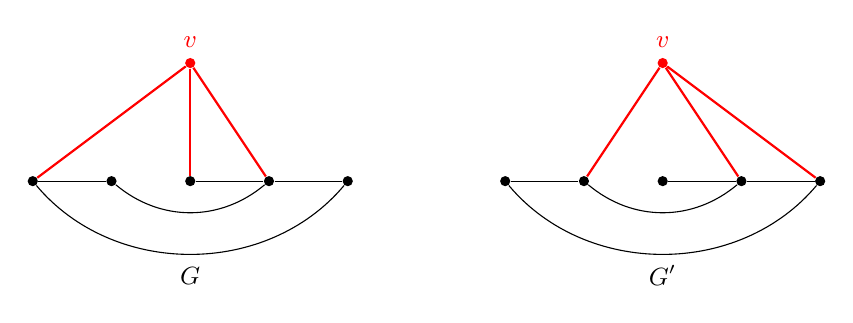
\begin{tikzpicture}[every node/.style={font=\small}, vtx/.style={circle, fill, inner sep=1.3pt}]
        \foreach \s/\name/\vedges in {0/G/{1,3,4}, 6/G'/{2,4,5}} {
            \begin{scope}[shift={(\s, 0)}]
                \node[vtx, red, label={[red]above:\(v\)}] (v) at (0, 1.5) {};
                \foreach \i in {1,...,5} \node[vtx] (u\i) at ({-2 + (\i - 1)}, 0) {};
                \draw (u1) -- (u2);
                \draw (u2) to[bend right=40] (u4);
                \draw (u3) -- (u4);
                \draw (u4) -- (u5);
                \draw (u1) to[bend right=50] (u5);
                \foreach \j in \vedges \draw[red, thick] (v) -- (u\j);
                \node at (0, -1.2) {\(\name\)};
            \end{scope}
        }
    \end{tikzpicture}
    \caption{\(G\) and \(G'\) differ only in the neighborhood of \(v\): the black edges, those not containing \(v\), are the same, while the red edges at \(v\) may change arbitrarily. A \(\delta\)-vertex-Lipschitz \(f\) has \(\abs{f(G) - f(G')} \le \delta\).}
    \label{fig:vertex-lipschitz}
\end{figure}

\begin{observation}
    Let \(f \colon \mathcal{G}_{n} \to \mathbb{R}\).
    \begin{enumerate}[(1)]
        \item If \(f\) is \(\delta\)-vertex-Lipschitz, then \(f\) is \(\delta\)-edge-Lipschitz.
        \item If \(f\) is \(\delta\)-edge-Lipschitz, then \(f\) is \(\delta(n-1)\)-vertex-Lipschitz.
    \end{enumerate}
\end{observation}

\begin{proof}
    (1) If \(G\) and \(G'\) differ in the single pair \(\{u, w\}\), then every pair in which they differ contains \(u\), so they differ only in the neighborhood of \(u\), and \(\abs{f(G) - f(G')} \le \delta\).

    (2) Suppose every pair in \(E(G) \mathbin{\triangle} E(G')\) contains \(v\). There are only \(n - 1\) pairs containing \(v\), so \(E(G) \mathbin{\triangle} E(G') = \{e_{1}, \ldots, e_{k}\}\) with \(k \le n - 1\). Switch these pairs one at a time: let \(H_{0} \coloneqq G\) and let \(H_{j}\) be \(H_{j-1}\) with the pair \(e_{j}\) switched (added if absent, removed if present). Then \(H_{k} = G'\), and consecutive graphs differ in a single pair, so by the triangle inequality
    \[
        \abs{f(G) - f(G')} \le \sum_{j=1}^{k} \abs{f(H_{j-1}) - f(H_{j})} \le k\delta \le (n-1)\delta . \qedhere
    \]
\end{proof}

Lipschitz conditions bound the increments of the Doob martingales from \autoref{sec:edge-exposure} and \autoref{sec:vertex-exposure}. The key point is that the pieces of information revealed are \emph{independent}. We prove this in a general form first.

\begin{lemma}[Bounded differences]\label{lem:bounded-differences}
    Let \(\eta_{1}, \ldots, \eta_{m}\) be independent random variables, each taking finitely many values, and let \(F\) be a function of \((\eta_{1}, \ldots, \eta_{m})\) such that
    \[
        \abs{F(\eta) - F(\eta')} \le \delta \qquad \text{whenever } \eta \text{ and } \eta' \text{ differ in a single coordinate}.
    \]
    Then the Doob martingale \(X_{i} \coloneqq \mathbb{E}[F(\eta) \mid \eta_{1}, \ldots, \eta_{i}]\) satisfies \(\abs{X_{i} - X_{i-1}} \le \delta\) for every \(1 \le i \le m\).
\end{lemma}

\begin{proof}
    Fix \(1 \le i \le m\). We split \(\eta\) into the past, the present and the future,
    \[
        \eta = (\underbrace{\eta_{1}, \ldots, \eta_{i-1}}_{\eta_{< i}}, \ \eta_{i}, \ \underbrace{\eta_{i+1}, \ldots, \eta_{m}}_{\eta_{> i}}) ,
    \]
    and write \(F(a, b, c)\) for the value of \(F\) when \(\eta_{< i} = a\), \(\eta_{i} = b\), \(\eta_{> i} = c\). Fix \(a\) and \(b\) with \(\mathbb{P}(\eta_{< i} = a, \eta_{i} = b) > 0\).

    \emph{Step 1: compute \(X_{i}\).} By independence, conditioning on \(\eta_{< i} = a\) and \(\eta_{i} = b\) does not change the distribution of \(\eta_{> i}\). So on the event \(\{ \eta_{< i} = a, \eta_{i} = b \}\),
    \[
        X_{i} = g(a, b) \coloneqq \sum_{c} \mathbb{P}(\eta_{> i} = c) \, F(a, b, c) ,
    \]
    the average of \(F\) over the unrevealed future.

    \emph{Step 2: compute \(X_{i-1}\).} Similarly, conditioning on \(\eta_{< i} = a\) does not change the joint distribution of \((\eta_{i}, \eta_{> i})\), under which \(\eta_{i}\) and \(\eta_{> i}\) are independent. So on the event \(\{ \eta_{< i} = a \}\),
    \[
        X_{i-1}
        = \sum_{b', c} \mathbb{P}(\eta_{i} = b') \, \mathbb{P}(\eta_{> i} = c) \, F(a, b', c)
        = \sum_{b'} \mathbb{P}(\eta_{i} = b') \, g(a, b') .
    \]
    So \(X_{i-1}\) is the weighted average of the possible values \(g(a, b')\) of \(X_{i}\).

    \emph{Step 3: compare two values of \(g\).} For any two values \(b, b'\) of \(\eta_{i}\), the inputs \((a, b, c)\) and \((a, b', c)\) differ only in coordinate \(i\), so \(\abs{F(a, b, c) - F(a, b', c)} \le \delta\) and
    \[
        \abs{g(a, b) - g(a, b')}
        \le \sum_{c} \mathbb{P}(\eta_{> i} = c) \, \abs{F(a, b, c) - F(a, b', c)}
        \le \delta \sum_{c} \mathbb{P}(\eta_{> i} = c)
        = \delta .
    \]

    \emph{Step 4: conclude.} On the event \(\{ \eta_{< i} = a, \eta_{i} = b \}\), using \(\sum_{b'} \mathbb{P}(\eta_{i} = b') = 1\),
    \[
        \abs{X_{i} - X_{i-1}}
        = \Bigl| \sum_{b'} \mathbb{P}(\eta_{i} = b') \bigl( g(a, b) - g(a, b') \bigr) \Bigr|
        \le \sum_{b'} \mathbb{P}(\eta_{i} = b') \, \delta
        = \delta .
    \]
    Every outcome lies in one such event, so \(\abs{X_{i} - X_{i-1}} \le \delta\) everywhere.
\end{proof}

\begin{fact}\label{fact:lipschitz-martingale}
    Let \(G \sim G(n, p)\) and \(f \colon \mathcal{G}_{n} \to \mathbb{R}\).
    \begin{enumerate}[(1)]
        \item If \(f\) is \(\delta\)-edge-Lipschitz, then the edge-exposure martingale of \(f(G)\) has \(\abs{X_{i} - X_{i-1}} \le \delta\).
        \item If \(f\) is \(\delta\)-vertex-Lipschitz, then the vertex-exposure martingale of \(f(G)\) has
        \(\abs{X_{i} - X_{i-1}} \le \delta\).
    \end{enumerate}
\end{fact}

\begin{proof}
    In both cases we apply \autoref{lem:bounded-differences} with \(F(\eta) = f(G)\), where \(G\) is the graph determined by \(\eta\).

    (1) Here \(\eta_{i} = \mathbbm{1}[e_{i} \in E(G)]\) for \(1 \le i \le \binom{n}{2}\). These are independent by the definition of \(G(n, p)\) (\autoref{def:gnp}). If \(\eta\) and \(\eta'\) differ only in coordinate \(i\), then the corresponding graphs differ only in the pair \(e_{i}\), so \(\abs{F(\eta) - F(\eta')} \le \delta\).

    (2) Here \(\eta_{i} = \bigl( \mathbbm{1}[\{j, i\} \in E(G)] \bigr)_{j < i}\) for \(1 \le i \le n\). Different \(\eta_{i}\) are indicators of disjoint sets of pairs, so they are independent. If \(\eta\) and \(\eta'\) differ only in coordinate \(i\), then the corresponding graphs differ only in pairs \(\{j, i\}\), all of which contain \(i\). So they differ only in the neighborhood of \(i\), and \(\abs{F(\eta) - F(\eta')} \le \delta\).
\end{proof}

\section{The Chromatic Number of \texorpdfstring{\(G(n,p)\)}{G(n,p)}}\label{sec:chi-gnp}

\begin{question}\label{q:chi-gnp}
    What is \(\chi(G(n,p))\)?
\end{question}

\subsection{Concentration: The Shamir--Spencer Theorem}\label{sec:shamir-spencer}

Before computing \(\chi(G(n,p))\), we show that it is concentrated around its mean.

\begin{theorem}[Shamir--Spencer, 1987]\label{thm:shamir-spencer}
    For every \(n\) and \(p\) there is a constant \(c = c(n, p)\) such that for \(G \sim G(n, p)\) and every \(\lambda > 0\),
    \[
        \mathbb{P}\bigl( \abs{\chi(G) - c} > \lambda \sqrt{n-1} \bigr) < 2 e^{-\frac{\lambda^{2}}{2}} .
    \]
    In fact one can take \(c = \mathbb{E}[\chi(G)]\).
\end{theorem}

\begin{proof}
    We apply \autoref{cor:azuma-general} with \(\delta = 1\) to the vertex-exposure martingale \(X_{0}, X_{1}, \ldots, X_{n}\) of \(f = \chi\).

    \emph{Step 1: \(\chi\) is \(1\)-vertex-Lipschitz.} Let \(G\) and \(G'\) differ only in the neighborhood of a vertex \(v\), so that \(G - v = G' - v\). Take a proper coloring of \(G\) with \(\chi(G)\) colors. Its restriction to \(V \setminus \{v\}\) is a proper coloring of \(G - v = G' - v\). Give \(v\) a new color, used nowhere else. The result is a proper coloring of \(G'\): an edge of \(G'\) either avoids \(v\), and is then an edge of \(G - v\), properly colored, or contains \(v\), whose color is unique. It uses \(\chi(G) + 1\) colors, so
    \[
        \chi(G') \le \chi(G) + 1 .
    \]
    Swapping the roles of \(G\) and \(G'\) gives \(\chi(G) \le \chi(G') + 1\), so \(\abs{\chi(G) - \chi(G')} \le 1\).

    \emph{Step 2: bounded increments.} By Step~1 and \autoref{fact:lipschitz-martingale}(2), \(\abs{X_{i} - X_{i-1}} \le 1\) for every \(1 \le i \le n\).

    \emph{Step 3: length \(n-1\).} Revealing vertex \(1\) reveals no pairs, so \(X_{1} = X_{0} = \mathbb{E}[\chi(G)] \eqqcolon c\) (\autoref{sec:vertex-exposure}). Drop \(X_{0}\) and consider
    \[
        c = X_{1}, X_{2}, \ldots, X_{n} ,
    \]
    a sequence of \(n - 1\) steps. It is still a martingale: since \(X_{0} = X_{1}\) is a constant, conditioning on \((X_{1}, \ldots, X_{i-1})\) is the same as conditioning on \((X_{0}, \ldots, X_{i-1})\). Its increments are bounded by \(1\) by Step~2, and its last value is \(X_{n} = \chi(G)\).

    \emph{Step 4: Azuma.} \autoref{cor:azuma-general} with \(m = n - 1\) and \(\delta = 1\) gives \(\mathbb{P}\bigl( \abs{\chi(G) - c} > \lambda \sqrt{n-1} \bigr) < 2 e^{-\lambda^{2}/2}\).
\end{proof}

\begin{remark}[What the theorem does and does not say]\label{rmk:shamir-spencer}
    \begin{itemize}
        \item \emph{The window.} Taking \(\lambda = \lambda(n) \to \infty\) slowly, \(\chi(G)\) lies in \([c - \lambda\sqrt{n}, c + \lambda\sqrt{n}]\) with high probability. For \(p = \frac{1}{2}\) we will see that \(\chi(G) \approx \frac{n}{2\log_{2} n}\), which is much larger than \(\sqrt{n}\). So, relative to its size, \(\chi\) is very concentrated.
        \item \emph{Vertex versus edge exposure.} \(\chi\) is also \(1\)-edge-Lipschitz, so edge exposure gives a window of order \(\sqrt{\binom{n}{2}} \approx \frac{n}{\sqrt{2}}\). Since \(\chi(G) \le n\) always, this says nothing. The shorter vertex-exposure martingale is what makes the theorem useful, as anticipated at the end of \autoref{sec:vertex-exposure}.
        \item \emph{The value.} The proof does not tell us \(c = \mathbb{E}[\chi(G)]\). Computing it is a separate problem, which we now start for \(p = \frac{1}{2}\).
    \end{itemize}
\end{remark}

\subsection{The Value for \texorpdfstring{\(p = \frac{1}{2}\)}{p = 1/2}: Lower Bound}\label{sec:chi-lower}

Let \(G \sim G(n, \frac{1}{2})\). By \autoref{prop:chromatic-bounds}(2),
\[
    \chi(G) \ge \frac{n}{\alpha(G)} ,
\]
so an \emph{upper} bound on the independence number \(\alpha(G)\) (\autoref{def:independence}) gives a lower bound on \(\chi(G)\).

\begin{question}\label{q:alpha-gnp}
    What is \(\alpha(G)\) for \(G \sim G(n, \frac{1}{2})\)?
\end{question}

\emph{First moment.} Let \(X_{k}\) be the number of independent sets of order \(k\) in \(G\). A \(k\)-set is independent iff all \(\binom{k}{2}\) pairs inside it are non-edges, which happens with probability \((\frac{1}{2})^{\binom{k}{2}}\). By \autoref{thm:linearity},
\[
    \mathbb{E}[X_{k}] = \binom{n}{k} \Bigl( \frac{1}{2} \Bigr)^{\binom{k}{2}} \eqqcolon f(k) .
\]
Subsets of independent sets are independent, so \(\alpha(G) \ge k\) iff \(X_{k} \ge 1\).

\begin{definition}\label{def:k0}
    Let \(k_{0} = k_{0}(n)\) be the smallest \(k\) with \(f(k) < 1\).
\end{definition}

This is well defined since \(f(n) = 2^{-\binom{n}{2}} < 1\) for \(n \ge 2\). Since \(f(0) = 1\) and \(f(1) = n\), we have \(k_{0} \ge 2\), and by minimality
\[
    f(k_{0}) < 1 \le f(k_{0} - 1) .
\]
So \(k_{0}\) is where the expected number of independent \(k\)-sets drops below \(1\).

\emph{Heuristic size of \(k_{0}\).} Using \(\binom{n}{k} \approx (\frac{ne}{k})^{k}\) (\autoref{rmk:binomial-estimates}),
\begin{equation}\label{eq:fk-approx}
    f(k) = \binom{n}{k} 2^{-\binom{k}{2}} \approx \Bigl( \frac{ne}{k} \Bigr)^{k} 2^{-\frac{k(k-1)}{2}} = \Bigl( \frac{ne}{k \, 2^{(k-1)/2}} \Bigr)^{k} .
\end{equation}
So \(f(k)\) crosses \(1\) roughly where the base is \(1\):
\[
    \frac{ne}{k_{0} \, 2^{(k_{0}-1)/2}} \approx 1
    \iff \frac{k_{0} - 1}{2} \approx \log_{2} \Bigl( \frac{ne}{k_{0}} \Bigr) = \log_{2} n - O(\log_{2} k_{0}) ,
\]
which gives \(k_{0} \sim 2 \log_{2} n\). The next lemma makes this precise.

\begin{lemma}\label{lem:k0-size}
    For \(n \ge 2\),
    \[
        2 \log_{2} n - 2 \log_{2} \log_{2} n - 1 < k_{0} < 2 \log_{2} n + 2 .
    \]
    In particular \(k_{0} = (2 + o(1)) \log_{2} n\).
\end{lemma}

\begin{proof}
    We use \(\bigl( \frac{n}{k} \bigr)^{k} \le \binom{n}{k} \le \bigl( \frac{ne}{k} \bigr)^{k}\) from \autoref{rmk:binomial-estimates}.

    \emph{Upper bound.} Let \(k \ge 2 \log_{2} n + 1\). Then \(\frac{k-1}{2} \ge \log_{2} n\), i.e.\ \(2^{(k-1)/2} \ge n\), and \(k \ge 3\). So, as in \eqref{eq:fk-approx} but with \(\le\),
    \[
        f(k) \le \Bigl( \frac{ne}{k \, 2^{(k-1)/2}} \Bigr)^{k} \le \Bigl( \frac{e}{k} \Bigr)^{k} < 1 .
    \]
    The least integer \(k \ge 2 \log_{2} n + 1\) is less than \(2 \log_{2} n + 2\), and it has \(f(k) < 1\). Hence \(k_{0} < 2 \log_{2} n + 2\).

    \emph{Lower bound.} Let \(\kappa \coloneqq 2 \log_{2} n - 2 \log_{2} \log_{2} n - 1\). If \(\kappa < 2\), the claim \(k_{0} > \kappa\) follows from \(k_{0} \ge 2\). Otherwise let \(1 \le k \le \kappa\). Then \(k \le 2 \log_{2} n\), and
    \[
        \frac{k - 1}{2} \le \frac{\kappa - 1}{2} = \log_{2} n - \log_{2}(2 \log_{2} n) ,
        \qquad\text{i.e.}\qquad
        2^{(k-1)/2} \le \frac{n}{2 \log_{2} n} \le \frac{n}{k} .
    \]
    So
    \[
        f(k) \ge \Bigl( \frac{n}{k} \Bigr)^{k} 2^{-\frac{k(k-1)}{2}} = \Bigl( \frac{n}{k \, 2^{(k-1)/2}} \Bigr)^{k} \ge 1 .
    \]
    Thus \(f(k) \ge 1\) for every \(k \le \kappa\) (for \(k = 0\), \(f(0) = 1\)), so the least \(k\) with \(f(k) < 1\) exceeds \(\kappa\).

    Finally, \(\frac{2 \log_{2} \log_{2} n + 2}{\log_{2} n} \to 0\), so both bounds are \((2 + o(1)) \log_{2} n\).
\end{proof}

\emph{How fast \(f\) drops.} Just above \(k_{0}\), \(f\) is already very small. To see this, compare consecutive terms. Since \(\binom{n}{k-1} / \binom{n}{k} = \frac{k}{n-k+1}\) and \(\binom{k}{2} - \binom{k-1}{2} = k - 1\),
\begin{equation}\label{eq:fk-ratio}
    \frac{f(k-1)}{f(k)}
    = \frac{\binom{n}{k-1}}{\binom{n}{k}} \cdot \frac{2^{-\binom{k-1}{2}}}{2^{-\binom{k}{2}}}
    = \frac{k}{n-k+1} \cdot 2^{k-1} .
\end{equation}
For \(k \sim 2 \log_{2} n\) we have \(2^{k-1} = n^{2 + o(1)}\) and \(\frac{k}{n-k+1} = n^{-1 + o(1)}\), because \(k = \Theta(\log n) = n^{o(1)}\). So
\[
    \frac{f(k-1)}{f(k)} = n^{1 + o(1)} \qquad \text{for } k \sim 2 \log_{2} n :
\]
near \(k_{0}\), increasing \(k\) by one divides \(f(k)\) by about \(n\). Since \(f(k_{0}) < 1\), this suggests \(f(k_{0} + 1) \le n^{-1 + o(1)}\). The next lemma gives an explicit bound.

\begin{lemma}\label{lem:fk0-plus-one}
    For \(n\) large, \(f(k_{0} + 1) < \dfrac{2 (\log_{2} n)^{2}}{n}\).
\end{lemma}

\begin{proof}
    If \(k_{0} + 1 > n\), then \(f(k_{0} + 1) = 0\). Otherwise apply \eqref{eq:fk-ratio} with \(k = k_{0} + 1\):
    \[
        \frac{f(k_{0})}{f(k_{0} + 1)} = \frac{k_{0} + 1}{n - k_{0}} \, 2^{k_{0}} \ge \frac{2^{k_{0}}}{n} ,
    \]
    since \(k_{0} + 1 \ge 1\) and \(n - k_{0} \le n\). By \autoref{lem:k0-size},
    \[
        2^{k_{0}} > 2^{2 \log_{2} n - 2 \log_{2} \log_{2} n - 1} = \frac{n^{2}}{2 (\log_{2} n)^{2}} ,
        \qquad\text{so}\qquad
        \frac{f(k_{0})}{f(k_{0} + 1)} > \frac{n}{2 (\log_{2} n)^{2}} .
    \]
    Since \(f(k_{0}) < 1\), this gives \(f(k_{0} + 1) < f(k_{0}) \cdot \frac{2 (\log_{2} n)^{2}}{n} < \frac{2 (\log_{2} n)^{2}}{n}\).
\end{proof}

\begin{proposition}\label{prop:alpha-upper}
    Let \(G \sim G(n, \frac{1}{2})\). With high probability \(\alpha(G) \le k_{0}\), and hence
    \[
        \chi(G) \ge \frac{n}{k_{0}} \ge (1 - o(1)) \frac{n}{2 \log_{2} n} .
    \]
\end{proposition}

\begin{proof}
    \(\alpha(G) \ge k_{0} + 1\) iff \(X_{k_{0}+1} \ge 1\). By \thmref{thm:markov} and \autoref{lem:fk0-plus-one},
    \[
        \mathbb{P}\bigl( \alpha(G) \ge k_{0} + 1 \bigr) = \mathbb{P}\bigl( X_{k_{0}+1} \ge 1 \bigr) \le \mathbb{E}[X_{k_{0}+1}] = f(k_{0} + 1) < \frac{2 (\log_{2} n)^{2}}{n} \longrightarrow 0 .
    \]
    So with high probability \(\alpha(G) \le k_{0}\), and then \(\chi(G) \ge \frac{n}{\alpha(G)} \ge \frac{n}{k_{0}}\). By \autoref{lem:k0-size}, \(k_{0} < 2 \log_{2} n + 2 = (1 + o(1)) \, 2 \log_{2} n\), so \(\frac{n}{k_{0}} \ge (1 - o(1)) \frac{n}{2 \log_{2} n}\).
\end{proof}

\subsection{Towards the Upper Bound}\label{sec:chi-upper-plan}

The lower bound came from the fact that every color class has at most \(\alpha(G) \approx 2 \log_{2} n\) vertices. To show that about \(\frac{n}{2 \log_{2} n}\) colors suffice, we would like to color \emph{greedily}: find an independent set of size about \(2 \log_{2} n\), give it color \(1\), remove it, find another in what is left, give it color \(2\), and so on (\autoref{fig:greedy-coloring}).

\begin{figure}[H]
    \centering
    \begin{tikzpicture}[every node/.style={font=\small}]
        \draw[thick, rounded corners] (0, 0) rectangle (6, 4.2);
        \node[anchor=west] at (6.2, 3.9) {\(G(n, \tfrac{1}{2})\)};
        \foreach \y/\col/\lab in {3.4/blue/1, 2.6/orange/2, 1.8/green!60!black/3} {
            \draw[\col, thick, rounded corners] (0.3, \y) rectangle (3.0, \y + 0.6);
            \node[\col] at (1.65, \y + 0.3) {\(\approx 2 \log_{2} n\)};
            \draw[\col, -Stealth] (-1.1, \y + 0.3) node[left] {color \(\lab\)} -- (0.25, \y + 0.3);
        }
        \node at (1.65, 1.35) {\(\vdots\)};
        \draw[gray, dashed, rounded corners] (3.4, 0.3) rectangle (5.7, 1.4);
        \node[gray, align=center, font=\footnotesize] at (4.55, 0.85) {few vertices left:\\one color each};
    \end{tikzpicture}
    \caption{Greedy coloring: repeatedly remove an independent set of size about \(2 \log_{2} n\) and give it a new color. If this works until few vertices remain, it uses about \(\frac{n}{2 \log_{2} n}\) colors, matching \autoref{prop:alpha-upper}.}
    \label{fig:greedy-coloring}
\end{figure}

The difficulty is that after a few rounds, the remaining vertices form a set that depends on \(G\), so we cannot simply treat what is left as a fresh random graph. Instead we ask that \emph{every} large set of vertices contains a large independent set.
\begin{itemize}
    \item \emph{What suffices.} Let \(m \coloneqq \bigl\lceil \frac{n}{(\log_{2} n)^{2}} \bigr\rceil\) and \(k = (2 - o(1)) \log_{2} n\). Suppose every \(S \subseteq [n]\) with \(\abs{S} \ge m\) has \(\alpha(G[S]) \ge k\). Then the greedy procedure can always continue while at least \(m\) vertices remain. Each round removes \(k\) vertices, so it runs for at most \(\frac{n}{k}\) rounds. The fewer than \(m\) leftover vertices get one new color each. In total
    \[
        \chi(G) \le \frac{n}{k} + m = (1 + o(1)) \frac{n}{2 \log_{2} n} + O\Bigl( \frac{n}{(\log_{2} n)^{2}} \Bigr) = (1 + o(1)) \frac{n}{2 \log_{2} n} .
    \]
    \item \emph{One set.} For a fixed \(S\) of size \(m\), \(G[S] \sim G(m, \frac{1}{2})\), and \(\log_{2} m = \log_{2} n - O(\log_{2} \log_{2} n) = (1 - o(1)) \log_{2} n\). So the analogue of \(k_{0}\) for \(G[S]\) is still \((2 - o(1)) \log_{2} n\), and the second moment method (\autoref{sec:second-moment-method}) shows that \(\alpha(G[S]) \ge k\) with high probability.
    \item \emph{All sets.} There are up to \(2^{n}\) sets \(S\), so for a union bound the failure probability for one \(S\) must be \(o(2^{-n})\). This is the situation of \autoref{sec:chernoff-motivation}: the second moment method gives a failure probability that is only polynomially small, while we need one that is exponentially small. This is where a martingale concentration inequality is needed.
\end{itemize}
Carrying this out gives the following theorem, which we prove next time.

\begin{theorem}[Bollob\'as, 1988]\label{thm:bollobas-chi}
    For \(G \sim G(n, \frac{1}{2})\), with high probability
    \[
        \chi(G) = (1 + o(1)) \frac{n}{2 \log_{2} n} .
    \]
\end{theorem}
